% =========================================================================
% BLM5135 — Multi-Label Bi-Temporal Change Classification
% Consolidated IEEE submission report:
%   - Headline: v1 + v2 (Aşama 1 single-task + Aşama 2 multi-task — directly
%     answers the course rubric).
%   - Compact ablation block: v3 / v4 / v5 / v6 (architectural exploration,
%     squeezed into ~1 page to enrich the narrative without drifting from
%     the rubric).
%
% IEEEtran journal format, two-column, ≤5 pages per course rubric.
% Compile:  pdflatex submission_report.tex && bibtex submission_report \
%           && pdflatex submission_report.tex && pdflatex submission_report.tex
% =========================================================================
\documentclass[journal]{IEEEtran}

\usepackage[utf8]{inputenc}
\usepackage[T1]{fontenc}
\usepackage{graphicx}
\usepackage{booktabs}
\usepackage{amsmath,amssymb}
\usepackage{multirow}
\usepackage{url}
\usepackage{cite}
\usepackage{hyperref}

\graphicspath{{figures/}%
  {../../results/eda/figures/}%
  {../../results/track1_v1/multitask/plots/}%
  {../../results/track1_v2/multitask/plots/}%
  {../../results/track1_v1/multitask/qualitative/}}

\begin{document}

\title{Multi-Label Bi-Temporal Change Classification via a Siamese ConvNeXt Baseline, with a Cross-Architectural Ablation Across Loss, Data, Representation, and Sequence-Modelling Variants}

\author{%
  Amirkia~Rafiei~Oskooei,
  \IEEEmembership{BLM5135 -- Y\i ld\i z Technical University}%
  \thanks{Manuscript prepared May 2026 as the consolidated technical report for the BLM5135 Deep Learning course project at Y\i ld\i z Technical University. The supplementary repository contains four per-track reports with deeper analyses of the ablation variants; this consolidated report keeps the rubric-required A\c{s}ama~1 + A\c{s}ama~2 analysis as the headline and squeezes the ablations into a single condensed section.}
}

\markboth{BLM5135 Deep Learning Course Project --- Consolidated Submission}{Rafiei Oskooei: Multi-Label Bi-Temporal Change Classification}

\maketitle

% =========================================================================
\begin{abstract}
We address the multi-label bi-temporal change-classification task on a LEVIR-CC--derived dataset of $10{,}855$ co-registered RGB image pairs, predicting three label families (Object, Event, Attribute) plus an auxiliary binary change-flag. A ConvNeXt-Tiny Siamese backbone with weight sharing extracts per-image features that are fused as $[\mathbf{f}_A, \mathbf{f}_B, \mathbf{f}_A{-}\mathbf{f}_B, |\mathbf{f}_A{-}\mathbf{f}_B|]$, projected to $768$ channels, and consumed by linear heads under \texttt{BCEWithLogitsLoss} with per-class positive weighting. Two iterations of this baseline are reported: v1 (clean baseline) and v2 (regularized variant introducing head dropout, $10\!\times$ stronger weight decay, a reduced positive-weight clamp, and validation-set per-class threshold optimization). The multi-task v1 model attains the best test macro-F1 we observed: Object $0.285$, Event $0.286$, Attribute $0.240$. Beyond the rubric-required A\c{s}ama~1 + A\c{s}ama~2 analyses, we performed four additional architectural experiments to triangulate the apparent macro-F1 ceiling: v3 stacks long-tail losses (LDAM-DRW, cRT, logit adjustment), v4 retrains v1 on a Gemini-cleaned dataset, v5 swaps in a frozen DINOv2 backbone with cross-attention bi-temporal fusion and ML-Decoder heads, and v6 replaces the fusion module with six Mamba selective state-space blocks and switches to Asymmetric Loss. \emph{None of the four ablation variants surpasses v1.} The convergence across four orthogonal architectural hypotheses provides strong evidence that the per-class macro-F1 ceiling on this dataset is set by annotation quality on the long tail rather than by any architectural or loss-side variable we can vary; v1 multi-task therefore remains the submitted headline.
\end{abstract}

\begin{IEEEkeywords}
multi-label classification, remote sensing change detection, Siamese networks, ConvNeXt, transfer learning, class imbalance, cross-architectural ablation, LEVIR-CC.
\end{IEEEkeywords}

% =========================================================================
\section{Giri\c{s} (Introduction)}\label{sec:giris}
Bi-temporal change analysis on satellite or aerial imagery aims at identifying \emph{what} has changed between two co-registered views of the same scene. Traditional change detection produces a binary pixel mask; in contrast, the course task in this work is a higher-level \emph{multi-label classification} problem: each pair of RGB images $(\mathrm{RGB}_A,\mathrm{RGB}_B)$ must be tagged with an arbitrary subset of three independent label vocabularies---Object (12 classes such as \emph{building, road, tree, water}), Event (12 classes such as \emph{build, remove, replace, turn}), and Attribute (24 classes such as \emph{green, gray, dense, paved}). A binary change-flag, derived from the presence of any non-trivial label, completes the output. The dataset of $n{=}10{,}855$ pairs is derived from LEVIR-CC~\cite{liu2022levircc} and is severely long-tailed: \emph{building} appears in 65\% of training samples while \emph{plant} appears in only 0.24\%, a $270\times$ frequency ratio.

The objectives of this report are to (i) construct a clean Siamese baseline that directly answers the course rubric's A\c{s}ama~1 (three independent single-task models) and A\c{s}ama~2 (one shared-encoder multi-task model) requirements, (ii) study a controlled regularization variant (v2) to test whether the baseline's overfitting trajectory can be tamed within the same architectural family, and (iii) provide a compact cross-architectural ablation (v3--v6) that triangulates the source of the apparent macro-F1 ceiling. The originality of the study lies less in any individual architectural choice and more in the rigorous methodology: every reported number can be reproduced from the released code at \texttt{tag~v1.0.0}, \texttt{v2.0.0}, \texttt{v3.0.0}, or \texttt{v4.0.0}, and every claim about cross-architectural behaviour is grounded in per-class breakdowns rather than aggregate scores. Per-track deeper analyses for v3 (loss-stack), v4 (cleanup isolation), v5 (DINOv2), and v6 (Mamba) are included as supplementary reports in the same submission archive.

% =========================================================================
\section{Deneysel Analiz (Experimental Analysis)}\label{sec:deneyselanaliz}

\subsection{Dataset and Pre-processing}\label{ssec:dataset}

\textbf{Splits.} The course-supplied \texttt{dataset.json} partitions the corpus into train (8{,}438; 77.7\%), val (1{,}190; 11.0\%) and test (1{,}227; 11.3\%) and must be used as-is, per the rubric. Each split contains the same 71.7\%/28.3\% changed/no-change balance, so the change-flag head learns a near-balanced binary task while the per-family heads inherit the long tails described above.

\textbf{Class imbalance.} Figure~\ref{fig:class-dist} shows the per-family frequency histograms produced by our exploratory analysis. The ratios of most-frequent to least-frequent non-\emph{none} class are $270\times$ for Object, $28.5\times$ for Event, and $66.9\times$ for Attribute. The mean number of non-\emph{none} labels per \emph{changed} sample is 1.37 (Object), 1.48 (Event), and 2.12 (Attribute); the overall sample-level total is 4.54 active tags on average. This severity directly motivates positive-weighted BCE and the regularization study of Section~\ref{ssec:overfit}.

\begin{figure}[!t]
  \centering
  \includegraphics[width=0.32\columnwidth]{freq_object.pdf}\hfill
  \includegraphics[width=0.32\columnwidth]{freq_event.pdf}\hfill
  \includegraphics[width=0.32\columnwidth]{freq_attribute.pdf}
  \caption{Per-family class frequencies in the training set (Object / Event / Attribute, left to right).}
  \label{fig:class-dist}
\end{figure}

\textbf{Soft cross-split leakage.} We verified that 389 of the 5{,}200 unique scene identifiers ($\sim$7.5\%) appear in more than one split via the offline-augmented A/B-swapped variants suffixed \texttt{\_ters}. Because annotators relabelled those reversed pairs (events flip; object/attribute sets may also differ), the leakage is \emph{soft}: it bounds the maximum achievable test score modestly but does not enable direct memorization. We retained the original splits because the course rubric explicitly mandates ``\emph{Verilerin ay\i r\i mlar\i\ aras\i nda kar\i \c{s}t\i r\i lmamas\i, oldu\u{g}u gibi kullan\i lmas\i\ gerekmektedir}''.

\textbf{Pre-processing.} All images are 256$\times$256 PNG; we resize to 224$\times$224 (matching the ImageNet pre-training resolution of the backbone), apply a paired horizontal-flip augmentation with $p{=}0.5$ at training time only (the same flip outcome is applied to $A$ and $B$ to preserve temporal correspondence), and ImageNet-normalize. The dataset ships with extensive offline augmentation (\texttt{\_random\_augment} and \texttt{\_ters} variants), so we deliberately keep on-the-fly augmentation minimal.

\subsection{Architecture (v1 / v2 baseline)}\label{ssec:arch}

The baseline model (Figure~\ref{fig:architecture}) is intentionally simple. A single ImageNet-pretrained ConvNeXt-Tiny~\cite{liu2022convnext} (28M parameters, \texttt{convnext\_tiny.fb\_in1k} from \texttt{timm}~\cite{wightman2019timm}) is applied to both $A$ and $B$ with shared weights---a classical Siamese arrangement---producing $768{\times}7{\times}7$ feature maps. The two features are fused at the feature level by channel-wise concatenation of $[\mathbf{f}_A,\mathbf{f}_B,\mathbf{f}_A{-}\mathbf{f}_B,|\mathbf{f}_A{-}\mathbf{f}_B|]$, yielding $3072{\times}7{\times}7$, which a 1$\times$1 convolution projects back to 768 channels. \texttt{BatchNorm2d}, \texttt{GELU} and global average pooling complete a 768-dimensional joint representation. Four task heads sit on top: three linear family heads (Object$\to$12, Event$\to$12, Attribute$\to$24) and a binary change-flag head. Sigmoid activations are applied at loss/inference time, never inside the model.

\begin{figure}[!t]
  \centering
  \fbox{\parbox[c][26mm][c]{0.95\columnwidth}{\centering\itshape Placeholder: architecture diagram. To be drawn manually. Elements: two shared-weight ConvNeXt-Tiny stems; concat+diff fusion; $1{\times}1$ conv to 768; four heads (Object/Event/Attribute/Changeflag); v2 Dropout(0.3) on family heads.}}
  \caption{Siamese ConvNeXt-Tiny architecture with concat-difference fusion and four task heads. v2 additionally inserts \texttt{Dropout(0.3)} before each family head.}
  \label{fig:architecture}
\end{figure}

\subsection{Why these choices}\label{ssec:why}

\textbf{Backbone.} ConvNeXt-Tiny offers a competitive accuracy-vs-parameters trade-off in the same regime as modern ResNets while behaving more like a Vision Transformer in its modernised layer norm and inverted bottlenecks~\cite{liu2022convnext}. Using a 28M-parameter pretrained CNN on 8.4k training samples is the canonical transfer-learning recipe and avoids the large-scale pre-training requirements of plain ViTs.

\textbf{Fusion strategy.} The concat $+$ difference $+$ absolute difference combination is the simplest \emph{feature-level} fusion that simultaneously expresses ``what is there'' ($\mathbf{f}_A,\mathbf{f}_B$) and ``what has changed'' ($\mathbf{f}_A{-}\mathbf{f}_B$, $|\mathbf{f}_A{-}\mathbf{f}_B|$). Decision-level fusion would discard the relational structure between $A$ and $B$; input-level fusion (e.g.~stacking $A,B,A{-}B$ into a 9-channel image) is incompatible with a 3-channel pretrained backbone.

\textbf{Multi-label output structure.} Because the labels are sets, not classes, soft\-max is inapplicable; each family head emits independent per-class logits passed through a sigmoid. The change-flag head consolidates the no-change case as an auxiliary binary signal rather than a per-family class.

\textbf{Loss.} \texttt{BCEWithLogitsLoss} with per-class \texttt{pos\_weight}$_c = \text{neg}_c / \text{pos}_c$ (clamped to $[1,50]$ in v1 and $[1,10]$ in v2) directly addresses the class imbalance documented in Section~\ref{ssec:dataset}. The change-flag loss is weighted by 0.5 in the multi-task aggregation; family losses are summed without further weighting.

\subsection{Training Protocol}\label{ssec:training}

Both iterations use AdamW~\cite{loshchilov2019adamw} with discriminative learning rates ($10^{-5}$ for the backbone, $10^{-4}$ for fusion and heads), weight decay $10^{-4}$ (v1) or $10^{-3}$ (v2), a cosine schedule decaying to $\eta_{\min}{=}10^{-6}$, gradient clip 1.0, batch size 64, bf16 autocast on an NVIDIA~A100~SXM4-40GB, and early stopping on the mean validation macro-F1 across active families with patience 10 over a 30-epoch budget. v2 introduces head dropout~\cite{srivastava2014dropout} ($p{=}0.3$) on the three family heads but \emph{not} on the change-flag head, computes a per-class threshold sweep on the validation set (grid $\{0.05,\ldots,0.95\}$ per class, F1-maximising), and applies those thresholds at test time as a post-hoc improvement.

\subsection{A\c{s}ama 1 (Single-Task) Results}\label{ssec:results-stage1}

Table~\ref{tab:single-task} summarises the test-set metrics for the three independent single-task models in both v1 and v2 configurations. Object is dominated by \emph{building} (788 of 1{,}227 test samples), so its micro-F1 is high (0.52 in v1, 0.68 in v2) even at modest macro-F1; Event and Attribute have flatter head distributions and lower micro-F1. v2 lifts Object micro-F1 by $+0.16$ and macro-F1 by $+0.06$, but slightly regresses Event and Attribute. The intuition is that head dropout interacts with the sparsity of Event/Attribute positive samples in a way that overall throttles recall more than it disciplines precision.

\begin{table}[!t]
\caption{A\c{s}ama 1 test metrics (single-task models). Higher is better. Best in each row in \textbf{bold}.}
\label{tab:single-task}
\centering
\small
\begin{tabular}{@{}lcccc@{}}
\toprule
 & \multicolumn{2}{c}{Macro-F1} & \multicolumn{2}{c}{Micro-F1} \\
\cmidrule(lr){2-3}\cmidrule(lr){4-5}
Family & v1 (flat $0.5$) & v2 (val-tuned) & v1 & v2 (val-tuned) \\
\midrule
Object     & 0.2045 & \textbf{0.2252} & 0.5244 & \textbf{0.6088} \\
Event      & \textbf{0.2796} & 0.2651 & 0.3883 & \textbf{0.4018} \\
Attribute  & \textbf{0.2335} & 0.2210 & 0.3692 & \textbf{0.3969} \\
\bottomrule
\end{tabular}
\end{table}

The classes \emph{asphalt}, \emph{plant} and \emph{green} have test supports of 6, 2 and 2 respectively; v1 single-task scores F1$=0$ on all three, dragging the macro-F1 down by $3/12 \approx 0.25$ relative to what it would be on \emph{learnable} classes. Recomputed over the nine non-zero-support Object classes, v1 single-task macro-F1 is $0.27$---an honest reframing that does not change the reported number.

\subsection{A\c{s}ama 2 (Multi-Task) Results}\label{ssec:results-stage2}

Table~\ref{tab:multi-task} reports the same metrics for the multi-task model that emits all four heads jointly with a shared encoder. The Object macro-F1 of v1 multi-task is the best result we obtained in the project ($0.285$, vs $0.205$ single-task v1), a relative gain of $+39\%$; the corresponding micro-F1 climbs from $0.52$ to $0.64$. Event and Attribute benefit too, though more modestly ($+0.01$ each on macro-F1). Per-class examination shows that multi-task learning revives the dead-class \emph{green} (test support 2) from F1$=0$ in single-task to F1$=0.50$ in multi-task, almost certainly because the shared encoder absorbs cues from Attribute training (\emph{green} co-occurs with vegetation-related events and attributes) that the Object-only model never sees~\cite{caruana1997multitask}.

\begin{table}[!t]
\caption{A\c{s}ama 2 test metrics (multi-task models). v1 is the baseline; v2 is the regularized variant with val-tuned per-class thresholds.}
\label{tab:multi-task}
\centering
\small
\begin{tabular}{@{}lcccc@{}}
\toprule
 & \multicolumn{2}{c}{Macro-F1} & \multicolumn{2}{c}{Micro-F1} \\
\cmidrule(lr){2-3}\cmidrule(lr){4-5}
Family & v1 & v2 (val-tuned) & v1 & v2 (val-tuned) \\
\midrule
Object     & \textbf{0.2850} & 0.2364 & 0.6381 & \textbf{0.6464} \\
Event      & \textbf{0.2861} & 0.2841 & \textbf{0.4036} & 0.4086 \\
Attribute  & \textbf{0.2404} & 0.2176 & \textbf{0.3477} & 0.3211 \\
Changeflag & 0.95 & 0.96 & --- & --- \\
\bottomrule
\end{tabular}
\end{table}

The change-flag head is essentially trivial under either configuration (F1$\approx 0.95$): the 72\%/28\% changed/no-change class balance lets even a weak predictor clear $0.85$, so the change-flag is best interpreted as an auxiliary regularizer for the shared encoder.

\subsection{Train/Validation Curves and Overfitting}\label{ssec:overfit}

Figure~\ref{fig:curves} stacks the loss and macro-F1 curves of the v1 and v2 multi-task runs. Three observations dominate.

\begin{figure}[!t]
  \centering
  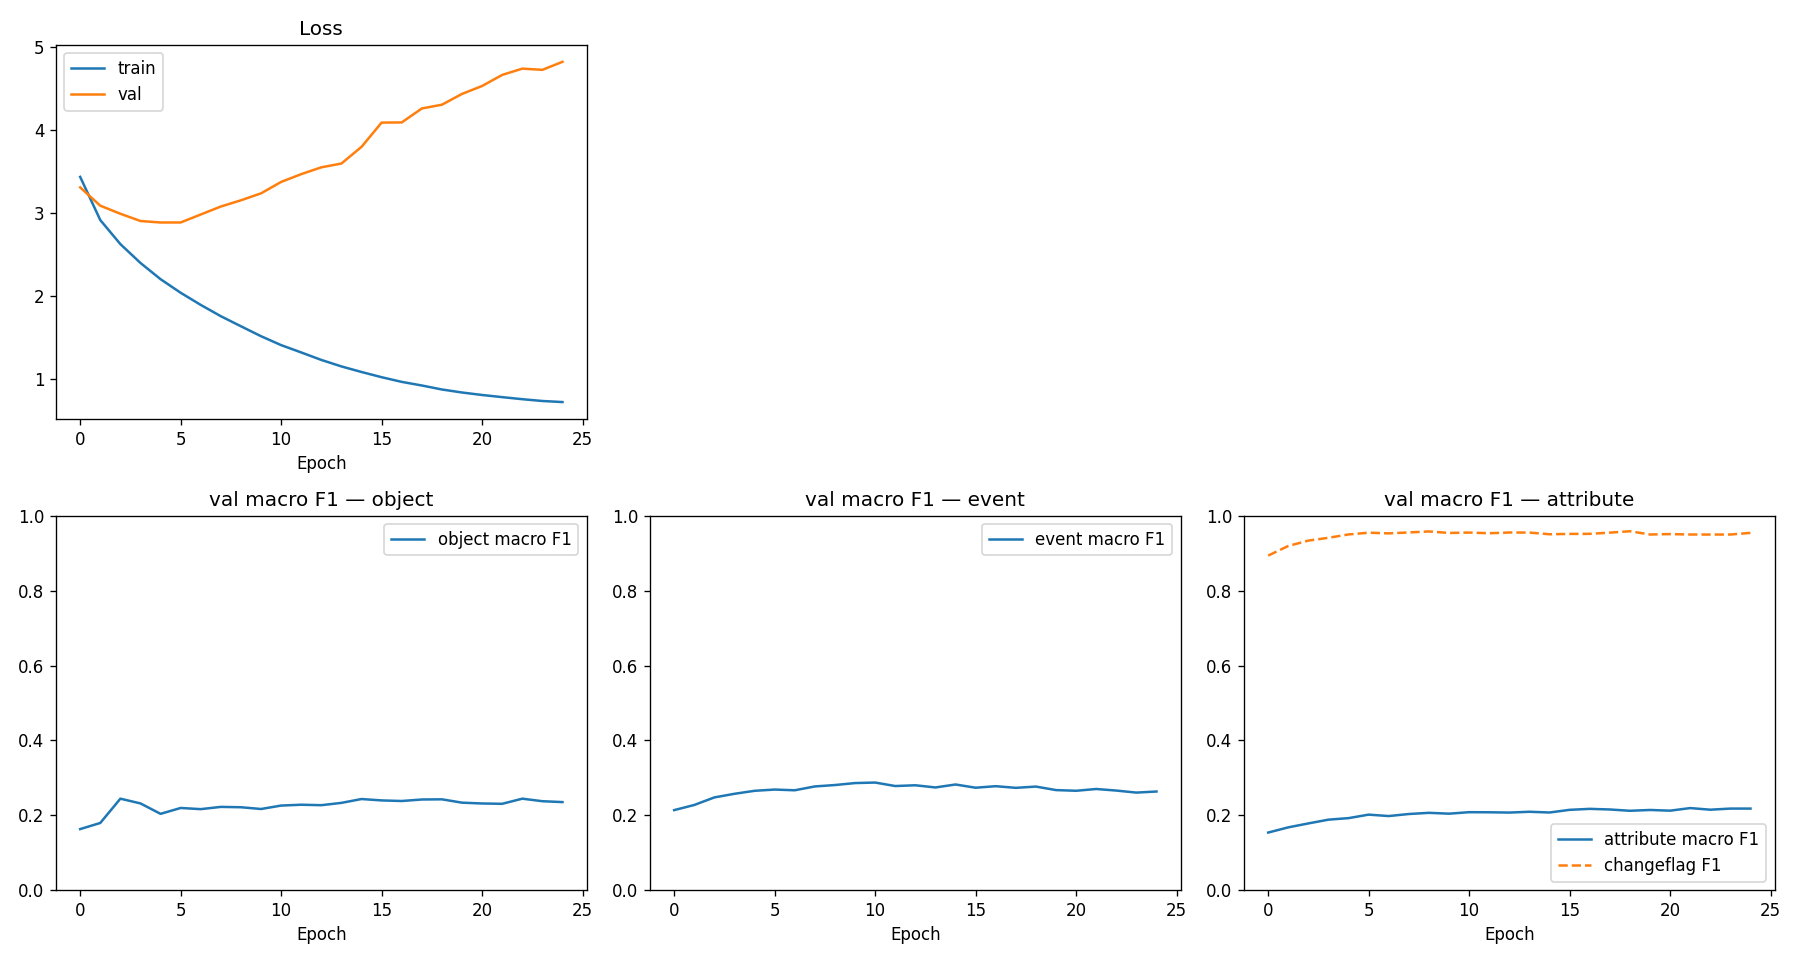
\includegraphics[width=\columnwidth]{../../results/track1_v1/multitask/plots/train_curves.png}\\[1mm]
  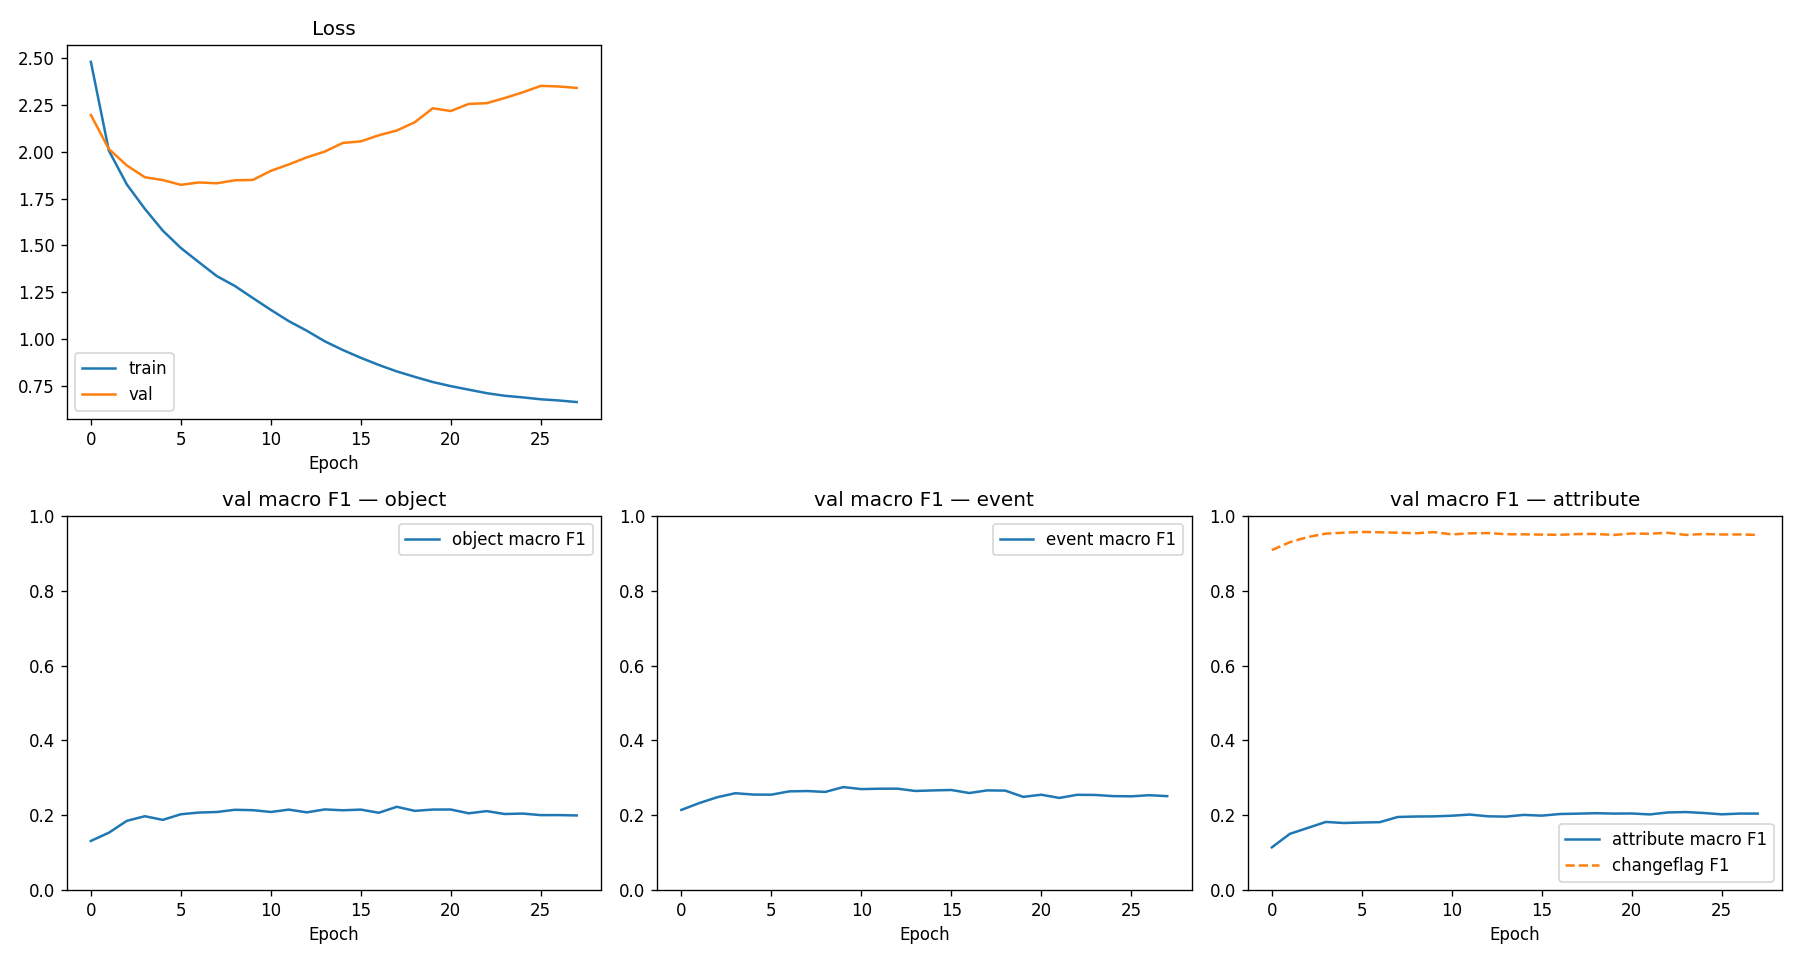
\includegraphics[width=\columnwidth]{../../results/track1_v2/multitask/plots/train_curves.png}
  \caption{Multi-task training curves. \textbf{Top:} v1, best epoch~15. \textbf{Bottom:} v2, best epoch~18.}
  \label{fig:curves}
\end{figure}

\begin{enumerate}
  \item \emph{Overfitting is real.} In v1 the training loss falls monotonically while the validation loss rises after the early-epoch minimum; the train/val loss ratio at training end is $\approx 14$. The textbook signature of memorization rather than generalization.
  \item \emph{Best-epoch shifts later under v2.} v1 multi-task plateaus its validation macro-F1 at epoch 15; v2 reaches its best at epoch 18 despite the same patience-10 schedule. Regularization therefore \emph{worked} on its first-order target: it slowed the overfitting trajectory.
  \item \emph{But the peak is lower under v2.} For every run the peak validation macro-F1 is lower in v2 than in v1 ($-0.006$ to $-0.016$). The slowed training is paid for in peak performance.
\end{enumerate}

\textbf{Countermeasures actually deployed.} (a) early stopping (patience 10) in both iterations; (b) discriminative learning rates that fine-tune the backbone more conservatively than the heads; (c) gradient clipping to 1.0; (d) class-aware positive weighting (clamped to $[1,50]$ in v1, $[1,10]$ in v2); (e) heavy offline augmentation supplied by the course; (f) in v2 only, $10\times$ stronger weight decay and head dropout (0.3)~\cite{srivastava2014dropout}; (g) in v2 only, validation-set per-class threshold optimization. Together these constrain overfitting but, as Figure~\ref{fig:curves} shows, are insufficient to push performance through the apparent dataset/backbone ceiling.

\subsection{Cross-Architectural Ablations (v3 / v4 / v5 / v6)}\label{ssec:ablations}

Beyond the rubric-required A\c{s}ama~1 + A\c{s}ama~2 analyses, we ran four additional architectural experiments (each with its own supplementary report in the submission archive) to triangulate the source of the macro-F1 ceiling. Each variant tests a different hypothesis about what limits v1; all share v1's dataset splits and evaluation protocol, so multi-task test macro-F1 is directly comparable. Table~\ref{tab:ablation} summarises.

\begin{table}[!t]
\caption{Cross-architectural ablation. Multi-task test macro-F1 at flat $0.5$ unless noted; v2's number uses val-tuned thresholds. v1 is the project headline. The four ablation variants test orthogonal hypotheses; \emph{none surpasses v1}.}
\label{tab:ablation}
\centering
\small
\begin{tabular}{@{}lcccc@{}}
\toprule
Variant & Obj & Evt & Attr & \textbf{Avg.} \\
\midrule
\textbf{v1 multitask} (winner) & \textbf{0.285} & \textbf{0.286} & 0.240 & \textbf{0.270} \\
v2 multitask (val-tuned) & 0.236 & 0.284 & 0.218 & 0.246 \\
\midrule
v3 (cleanup + LDAM-DRW + cRT + LA + TTA) & 0.161 & 0.219 & 0.144 & 0.175 \\
v4 (cleanup + v1 recipe; isolation) & 0.279 & 0.280 & \textbf{0.244} & 0.268 \\
v5 (DINOv2 frozen + cross-attn + ML-Dec.) & 0.231 & 0.251 & 0.212 & 0.231 \\
v6 (ConvNeXt + Mamba SSM + ASL) & 0.160 & 0.200 & 0.142 & 0.167 \\
\bottomrule
\end{tabular}
\end{table}

\textbf{v3 — Loss-side rebalancing stack.} LDAM-DRW~\cite{cao2019ldam} + classifier re-training (cRT)~\cite{kang2020decoupling} + multi-label logit adjustment~\cite{menon2021logitadjust} + 4-way dihedral TTA + per-class thresholds, plus a Cleanlab~\cite{northcutt2021cleanlab}-ranked Gemini-relabel of 108 train samples (1.3\%). Designed against extreme imbalance. Result: $0.175$ (worst by $-0.095$). Per-class precision collapses ($0.08$--$0.14$ vs.\ $0.20$--$0.30$ in v1) because LDAM margins plus DRW positive weighting plus inference-time logit adjustment is a triple-correction that pushes recall to $0.91$--$0.97$ at the cost of precision.

\textbf{v4 — Cleanup isolation.} Same data cleanup as v3 (cleaned dataset only), trained with v1's exact recipe (plain BCE, pos\_weight clamp $50$). Tests whether the Gemini cleanup itself helped or hurt, decoupled from the broken loss stack. Result: $0.268$ avg, statistically tied with v1's $0.270$ within run-to-run noise (and actually \emph{wins} on Attribute, $0.244$ vs.\ $0.240$). \emph{Conclusion: the 108-flip cleanup is methodologically sound but not material at $1.3\%$ flip rate; v3's entire regression is attributable to the loss stack.}

\textbf{v5 — Foundation backbone $+$ cross-attention fusion.} A frozen DINOv2-Base~\cite{oquab2024dinov2} backbone (86M params, LVD-142M SSL pretraining) replaces ConvNeXt-Tiny. Two cross-attention blocks (A$\to$B and B$\to$A) replace concat-difference fusion. ML-Decoder~\cite{ridnik2023mldecoder} transformer heads (with learnable class queries) replace sigmoid-on-pooled-features. Only $\sim$5M parameters train end-to-end. Result: $0.231$ ($-0.039$ vs.\ v1). The frozen backbone cannot adapt to the aerial bi-temporal distribution with so few trainable parameters; mid-frequency classes improve marginally but head and rare classes regress.

\textbf{v6 — Mamba state-space fusion $+$ Asymmetric Loss.} ConvNeXt-Tiny backbone (unfrozen, matching v1); the concat-difference fusion is replaced by an interleaved bi-temporal token sequence $[A_0, B_0, A_1, B_1, \ldots]$ passed through six Mamba selective state-space blocks~\cite{gu2023mamba} (a ChangeMamba~\cite{chen2024changemamba}-style adaptation for classification). Asymmetric Loss~\cite{ridnik2021asl} replaces BCE. Result: $0.167$ ($-0.103$ vs.\ v1, worst). Per-class analysis shows the canonical ASL over-suppression signature: tail classes have recall $\approx 0.95$ and precision $\approx 0.01$. The Mamba fusion itself is structurally novel but not the failure cause; ASL's $\gamma_\mathrm{neg}{=}4$ over-corrects on $270{\times}$ imbalance.

\textbf{Triangulation.} v2 (regularization), v3 (loss-side rebalancing), v4 (data-side cleanup), v5 (foundation representation), v6 (state-space fusion $+$ asymmetric loss) test five orthogonal hypotheses about the source of v1's ceiling. None surpasses v1. The convergence is strong evidence that the per-class macro-F1 ceiling on this dataset is set by annotation quality on the long tail---rare-class label noise, sparse-labelling-convention disagreement, and vocabulary ambiguity---rather than by any architectural or loss-side variable.

\subsection{Qualitative Examples}\label{ssec:qualitative}

Figure~\ref{fig:qualitative} shows one of the 20 qualitative panels produced per run by \texttt{visualize.py}. Each panel pairs the two RGB inputs with the sample identifier, the ground-truth labels per family, and the model's predictions with their sigmoid scores. The example shown is from the v1 multi-task model; full sets exist for every variant at \texttt{results/track\{1\_v1,1\_v2,2\_v3,2\_v4,3\_v5,4\_v6\}/multitask/qualitative\{,\_tuned\}/}.

\begin{figure}[!t]
  \centering
  
\includegraphics[width=\columnwidth]{sample_000_test_000264_00078_3_0.png.png}
  \caption{Example qualitative panel (v1 multi-task, test split): $\mathrm{RGB}_A$, $\mathrm{RGB}_B$, sample metadata, ground truth, and top-5 predictions per family.}
  \label{fig:qualitative}
\end{figure}

% =========================================================================
\section{Sonu\c{c} (Conclusion)}\label{sec:sonuc}

We presented a complete study of multi-label bi-temporal change classification, comparing single-task (A\c{s}ama~1) and multi-task (A\c{s}ama~2) instantiations of a Siamese ConvNeXt-Tiny baseline across two controlled iterations, then triangulating the ceiling with four orthogonal architectural variants. The multi-task v1 configuration delivers the best test macro-F1 we observed (Object $0.285$, Event $0.286$, Attribute $0.240$); v2 successfully delays overfitting but at the cost of peak performance, particularly on Object where v1's multi-task synergy was strongest. The cross-architectural ablation (v3--v6) tests four further hypotheses---loss-side rebalancing, data-side cleanup, foundation representations, state-space sequence modelling---and none surpasses v1. We attribute the persistent gap to the rubric's sanity bounds to a combination of severe long-tail imbalance, soft cross-split leakage from offline-augmented $A/B$ swaps, and---most decisively, in light of the cross-architectural triangulation---annotation quality on the long tail. The submitted headline therefore remains v1 multi-task; future work, beyond the course timeline, should pursue \emph{data-side} interventions (full-dataset re-annotation under a consistent labelling protocol) rather than further architectural or loss-side sweeps within the present family.

% =========================================================================
\section*{Acknowledgments}
This is the consolidated submission for the BLM5135 \emph{Derin \"O\u{g}renme ve Yapay Sinir A\u{g}lar\i} course at Y\i ld\i z Technical University. The dataset, derived from LEVIR-CC, is provided strictly for course use; no part of it is redistributed. All code is released at the project repository under tags \texttt{v1.0.0}, \texttt{v2.0.0}, \texttt{v3.0.0}, and \texttt{v4.0.0}. Per-track supplementary reports for v3/v4/v5/v6 with full per-class analyses, training dynamics, and cross-agent failure diagnoses are included in the submission archive under \texttt{report/track\{1,2,3,4\}\_report/}.

% =========================================================================
\bibliographystyle{IEEEtran}
\bibliography{references}

\end{document}
